%%%%%%%%%%%%%%%%%%%%%%%%%%%%%%%%%%%%%%%%%%%%%%%%%%%%%%%%%%%%%%%%%%%%%%%%%%%%%%%%
%
% Chapter: Case Study: Payment Analysis For Business Intelligence
%
%%%%%%%%%%%%%%%%%%%%%%%%%%%%%%%%%%%%%%%%%%%%%%%%%%%%%%%%%%%%%%%%%%%%%%%%%%%%%%%%
\chapter{Payment History Analysis: A Case Study and Problem Statement} \label{ch:problem}
The payment history analysis case study has been provided by a local software company who wishes to remain anonymous. From this point on, we will 
refer to this company as ``CompanyX''.  CompanyX provides software tools for customer information management and record analysis for BI. CompanyX evaluates current and historical payment habits for each customer account and attempts to predict future payment patterns based on past trends. Successful prediction of whether a payment will be on-time, past-due, or delinquent may reduce administrative costs accrued by outsourcing delinquent accounts for payment collection.  For example, if a customer has always made late payments in the past, they can expect that the customer will continue to make payments, even if they are late, and thus avoid sending them to a collection agency. 

As they expand their services, CompanyX expects the number of customers to increase from several hundred to several \textit{thousand}. This is a major cause for concern because the amount and complexity of collected data will increase as well, forcing the storage and access of data from their current hardware system to a more sophisticated system. Adopting a new hardware system while maintaining their existing service can be expensive, time-consuming, and may compromise data integrity and service availability as data is transferred from the old system to the new. Because of the risks involved, the company would like to compare the viability of other systems before converting their entire business architecture. This project will address the two major concerns that arise as a consequence of the increasing data volume: \textit{data storage model} and the \textit{scalability of data analysis software}. Due to privacy rights, any records collected by the company cannot be used, so sample data sets must be generated as prerequisite for testing new system implementations.

Our research assesses potential open source data warehousing models for CompanyX.

\section{The Case Study}

\subsection{Data Storage and Relationship Model}
The data must be staged for data warehousing. During this process, the data is pruned and normalized to fit a chosen data storage model. In this case, CompanyX has selected an RDBMS for data management (deployed on a local, in-house server), which is used for both operational and warehousing purposes. For this, the data is normalized to include a(n):
\begin{enumerate}
 \item \texttt{Customer} tuple for each customer (Table~\ref{tbl:custtuple}),
 \item \texttt{Account} tuple for each customer account (Table~\ref{tbl:accttuple}),
 \item \texttt{Transaction} tuple for each account transaction (Table~\ref{tbl:trantuple}), and
 \item \texttt{StrategyHistory} tuple for each account strategy (Table~\ref{tbl:strategytuple}).
\end{enumerate}
Note that the referenced tables use a solid underline to identify the \underline{primary key} and a dashed underline to identify a \dashuline{foreign key}. The relationship model between the tables is described below and shown in Figure~\ref{fig:eer-model}. 
%-------------------------------------------------------------------------------
% List of databaset tables
%-------------------------------------------------------------------------------
\begin{description}
 %------------------------------------------------------------------------------
 % Customer Tuple
 %------------------------------------------------------------------------------
 \item [Customer:]
  The unique \textit{primary key} for the customer entity-type is the
  \texttt{CustomerNumber} attribute. Each customer entity stores the
  customer's social security number (\texttt{ssn}) and the first three digits
  of the customer's zip code (\texttt{zipcode3}).
  \begin{table}[ht]
  \caption{ Customer Tuple }
  \label{tbl:custtuple}
  \centerline{
  \begin{tabular}{|l|l|l|l|l|}
   \hline
   \underline{CustomerNumber} & FirstName & LastName & Ssn & ZipCode3 \\
   \hline
  \end{tabular}
  }
 \end{table}
 %------------------------------------------------------------------------------
 % Account Tuple
 %------------------------------------------------------------------------------
 \item [Account:] 
  The unique \textit{primary key} for the account entity-type is the \texttt{AccountNumber} attribute. Each account entity includes the date the account was opened (\texttt{opendate}) and is \textit{is-owned-by} a unique customer, which is referenced by a foreign key\\ (\texttt{CustomerNumber}).
 \begin{table}[ht]
  \caption{ Account Tuple }
  \label{tbl:accttuple}
  \centerline{
  \begin{tabular}{|l|l|l|}
   \hline
   \underline{AccountNumber} & OpenDate & \dashuline{CustomerNumber}\\
   \hline
  \end{tabular}
  }
 \end{table}
 %------------------------------------------------------------------------------
 % Transaction Tuple
 %------------------------------------------------------------------------------
 \item [Transaction:]
The transaction entity is a weak type which depends on the account entity. Each transaction entity \textit{is-owned-by} a unique account which is referenced by the \texttt{AccountNumber} key and includes the type of transaction (\texttt{TransactionType} $\in$ \{\texttt{charge}, \texttt{adjustment}, \texttt{payment}\}), the date of the transaction (\texttt{TransactionDate}), and the amount of the transaction (\texttt{TransactionAmount}). The unique identifier is a \textit{composite key} composed of the \texttt{AccountNumber} reference, \texttt{TransactionType}, \texttt{TransactionDate}, and \texttt{TransactionAmount}.
 \begin{table}[ht]
  \caption{ Transaction Tuple }
  \label{tbl:trantuple}
  \centerline{
  \begin{tabular}{|l|l|l|l|}
   \hline
   \underline{\dashuline{AccountNumber}} & \underline{TransactionType} &
   \underline{TransactionDate}& \underline{TransactionAmount}\\
   \hline
  \end{tabular}
  }
 \end{table}
 %------------------------------------------------------------------------------
 % StrategyHistory Tuple
 %------------------------------------------------------------------------------
 \item [StrategyHistory:]
  The strategy history entity-type also depends on the account entity. Each
  strategy history entity \textit{is-owned-by} a unique account which is
  referenced by the \texttt{AccountNumber} key and includes the name of the strategy (\texttt{StrategyName} $\in$ \{\texttt{Good
  Standing}, \texttt{Bad Debt}\}) and the start date of the strategy
  (\texttt{StrategyStartDate}). The unique identifier is a \textit{composite key} composed of the \texttt{AccountNumber}
  reference, \texttt{StrategyName}, and \texttt{StrategyStartDate}.
 \begin{table}[ht]
  \caption{ StrategyHistory Tuple }
  \label{tbl:strategytuple}
  \centerline{
  \begin{tabular}{|l|l|l|}
   \hline
   \underline{\dashuline{AccountNumber}} & \underline{StrategyName} &
   \underline{StrategyStartDate}\\ 
   \hline
  \end{tabular}
  }
 \end{table}
\end{description}

%-------------------------------------------------------------------------------
% PaymentAnalysis Schema
%-------------------------------------------------------------------------------
\begin{figure}[ht]
\begin{center}
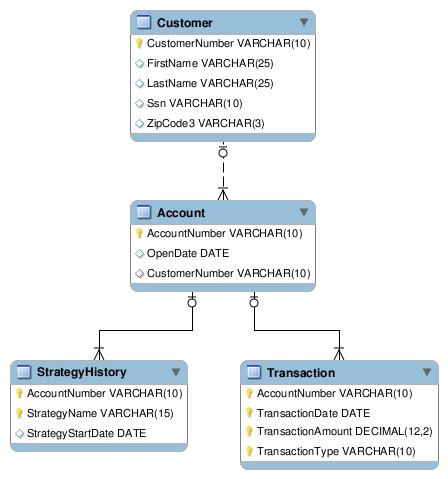
\includegraphics[width=\textwidth]{../images/account-history-schema.jpg}
\end{center}
\caption{Account history data entity-relationship model}
\label{fig:eer-model}
\end{figure}

\subsection{Data Access Model}
In order for CompanyX to use the data as input for their payment prediction algorithms, they must extract and prepare \textit{meaningful} data from the database. Data retrieval is achieved through join, aggregate, and other relevant SQL queries to the database. The resulting output of these queries must supply the input parameters for the prediction algorithms:
\begin{itemize}
 \item Aggregate charge, adjustment, and payment sums of historical transaction data.
 \item Aggregate payment sums of historical transaction data for all previous accounts owned by the same customer.
\end{itemize}

For a complete summary of CompanyX's expected output see Table~\ref{tbl:histtuple}.
{
\small
\begin{table}[ht]
 \caption{ Expected Result Tuple - Attribute descriptions }
 \label{tbl:histtuple}
 \centerline{
 \begin{tabular}{|l|p{7.5cm}|}
  \hline
  \textit{AccountNumber} & unique Account identifier\\ 
  \hline  
  \textit{OpenDate} & date the Account was opened by Customer\\
  \hline  
  \textit{ZipCode3} & first three digits of Customer's zip code\\
  \hline
  \textit{TotalCharges} & sum of all Charge transactions on Account\\
  \hline  
  \textit{TotalAdjustments} & sum of all Adjustment transactions on Account\\
  \hline
  \textit{AdjustedTotalCharges} & sum of TotalCharges and TotalAdjustments\\
  \hline
  \textit{TotalGoodStandingPayments30Day} & negative of sum of all payment
  transactions on account between 1 and 30 days after Good Standing strategy
  start date but before Bad Debt strategy start date\\
  \hline
  \textit{TotalGoodStandingPayments60Day} & same as above, but between 1 and 60
  days\\
  \hline
  \textit{TotalGoodStandingPayments90Day} & same as above, but between 1 and 90
  days\\
  \hline
  \textit{BadDebtTransferBalance} & sum of all transactions on account up
  through "Bad Debt" strategy start date\\
  \hline
  \textit{TotalBadDebtPayments30Day} & negative sum of all payment transactions
  on account between 1 and 30 days after Bad Debt strategy start date\\
  \hline
  \textit{TotalBadDebtPayments60Day} & same as above, but between 1 and 60
  days\\
  \hline
  \textit{TotalBadDebtPayments90Day} & same as above, but between 1 and 90
  days\\
  \hline
  \textit{PreviousAccountCount} & number of accounts with open date prior to
  this account's open date which have a customer with the same SSN\\
  \hline  
  \textit{PreviousAccountGoodStandingCharges} & sum of all charge transactions
  occurring prior to this account's open date on accounts which have a
  customer with the same SSN (not same account) which occurred while other
  accounts were at or after Good Standing strategy start date but before
  other accounts were at Bad Debt strategy start date\\
  \hline
  \textit{PreviousAccountGoodStandingAdjustments} & sum of all adjustments that
  occurred during Good Standing strategy for past accounts\\
  \hline
  \textit{PreviousAccountGoodStandingPayments} & sum of all Payments that
  occurred during Good Standing strategy for past accounts\\
  \hline
  \textit{PreviousAccountBadDebtPayments} & sum of all Payments that occurred
  during Bad Debt strategy for past accounts\\	
   \hline
  \end{tabular}
  }
 \end{table}
}

The first step of the retrieval process is to gather the transaction history data for each account, per strategy period. Recall that the relationships between account and transaction and customer and account are of \textit{one-to-many}. The total charges and adjustments do not depend on the strategy period, so these fields only require data stored in the \texttt{Transaction} table. However, because the account payments are subdivided into thirty, sixty and ninety day good standing and bad debt strategy periods, both the \texttt{StrategyHistory} and \texttt{Transaction} tables are required to select transactions per period. The process can be broken into these simplified steps:
\begin{enumerate}
 \item Join the \texttt{Account} and \texttt{Customer} tables to associate customer data with each account.
 \item Join the \texttt{Account} and \texttt{Transaction} tables to collect aggregate sums of \texttt{charge} and \texttt{adjustment} transactions, per account.
 \item Join the \texttt{Account}, \texttt{StrategyHistory} and \texttt{Transaction} tables to collect aggregate sums of \texttt{payment} transactions by strategy history type.
\end{enumerate}

At this point, the attributes stored in the result entity for an account include the customer data, total charges and adjustments, and payments per
strategy period. The next step will aggregate the transactions for all previous accounts with the same \texttt{ssn}. The result depends on the \texttt{OpenDate} of each account with the same \texttt{CustomerNumber} to determine if it is a previous account. If the account was opened before the
current account, then the result will depend on the \texttt{Transaction} and \texttt{StrategyHistory} tables. The process can be broken into these simplified steps:
\begin{enumerate}
 \item Determine the \texttt{ssn} of each account by joining \texttt{Account} and \texttt{Customer}.
 \item Left outer join \texttt{Account} table with itself on \texttt{ssn} and select accounts where \texttt{OpenDate} of the joined account is before the \texttt{OpenDate} of the left outer account.
 \item Join the result of the previous step with \texttt{StrategyHistory} and \texttt{Transaction} tables to collect aggregate sums of previous account
  transactions by transaction type, strategy history type, and account.
\end{enumerate}

%===============================================================================
% Subsection: Account Data Generation
%===============================================================================
\subsection{Account Data Generation}
To respect customer privacy, potential test data related to real-world customer accounts and transaction histories have been withheld. In order to provide us with a starting point, CompanyX used their expert knowledge of the data trends to compile a small sample of transactions, strategy histories, and customer data for 200 accounts. However, several thousand accounts are needed for an accurate comparison between the performance metrics of potential solutions and the current implementation. Therefore, we must generate our own test data. To maintain quality as the quantity increases,
the attributes of the generated data sets should adhere to the same probability distributions as the sample data. More detailed information about these
attributes are outlined in Chapter~\ref{ch:solution}.

\section{Problem Statement}
CompanyX is faced with challenges pertaining to Big Data:
\begin{enumerate}
 \item There is too much data to store on single machine.
 \item The database access times increase drastically as the amount and complexity of data accumulates over time.
\end{enumerate}
For this, we wish to know if we can use distributed model, such as Hadoop, without significant loss of performance on existing \textit{small} data sets, in order to prepare for the future \textit{big} data sets. In doing so, perhaps it is possible to achieve a performance gain on current and future data sets. So we know Hadoop performs well for Big Data analysis, but how will it perform in this particular case?

Thus, the goals of the research project for CompanyX are to:
\begin{itemize}
  \item Design and implement a scalable BI solution for extracting patterns in customer history data using existing open-source projects.
  \item Generate large sample data sets (hundreds of gigabytes) using Hadoop to compare the scalability of the MapReduce solution to the existing MySQL solution.
  \item Implement and compare a Hadoop MapReduce solution.
  \item Implement and compare a Hadoop Hive solution.
\end{itemize}
Therefore, we will address the following questions:
\begin{enumerate}
 \item At what scale of data (number of accounts or customers) does each solution out-perform the others?
 \item Will the existing data schema work with each solution?
 \item How much cost and effort will it take to deploy each solution?
\end{enumerate}